% !TeX root = Protokoll.tex
\subsection{Gegengekoppelter Verstärker}

\begin{table}[!h]
	\centering
	\begin{tabular}{ccc}
		\toprule
		Widerstand & Widerstand & Verhältnis\\
		$R_N$/\si{\kilo\ohm} & $R_1$/\si{\kilo\ohm} & $\frac{R_N}{R_1}$\\
\midrule
		\num{100(1)} & \num{100(1)} & \num{1.00(1)}\\
		\num{10.0(1)} & \num{100(1)} & \num{0.100(1)}\\
		\num{10.0(1)} & \num{32.0(3)} & \num{0.312(4)}\\
		\num{32.0(3)} & \num{10.0(1)} & \num{3.20(5)}\\
		\bottomrule
	\end{tabular}
	\caption{Werte der 4 Widerstandspaare, die für die unterschiedlichen Schaltungen des gegengekoppelten Verstärkers 
verwendet wurden. Zusätzlich angegeben ist das Verhältnis dieser beiden Widerstände. \label{tab:gegengekoppelt_widerstaende}}
\end{table}


\begin{table}[!h]
	\centering
	\begin{tabular}{ccc}
		\toprule
		Frequenz & Ausgangsspannung & Verstärkung\\
		$f$/\si{\kilo\hertz} & $U_A$/\si{\milli\volt} & $V$\\
\midrule
		\num{1.00(1)} & \num{78(5)} & \num{1.11(7)}\\
		\num{5.00(5)} & \num{72(5)} & \num{1.03(7)}\\
		\num{10.0(1)} & \num{57(5)} & \num{0.81(7)}\\
		\num{15.0(1)} & \num{45(5)} & \num{0.64(7)}\\
		\num{20.0(2)} & \num{37(5)} & \num{0.53(7)}\\
		\num{25.0(2)} & \num{31(5)} & \num{0.44(7)}\\
		\num{30.0(3)} & \num{25(5)} & \num{0.36(7)}\\
		\num{35.0(4)} & \num{25(5)} & \num{0.36(7)}\\
		\num{75.0(8)} & \num{20(5)} & \num{0.29(7)}\\
		\num{100(1)} & \num{15(5)} & \num{0.21(7)}\\
		\bottomrule
	\end{tabular}
	\caption{Messwerte der Frequenz und der Ausgangsspannung der ersten Schaltung eines gegengekoppelten Verstärkers.
            Zusätzlich ist die Verstärkung dieser Schaltung angegeben. \label{tab:gegengekoppelter_verstaerker_1}}
\end{table}

\FloatBarrier
\begin{figure}[!h]
\centering
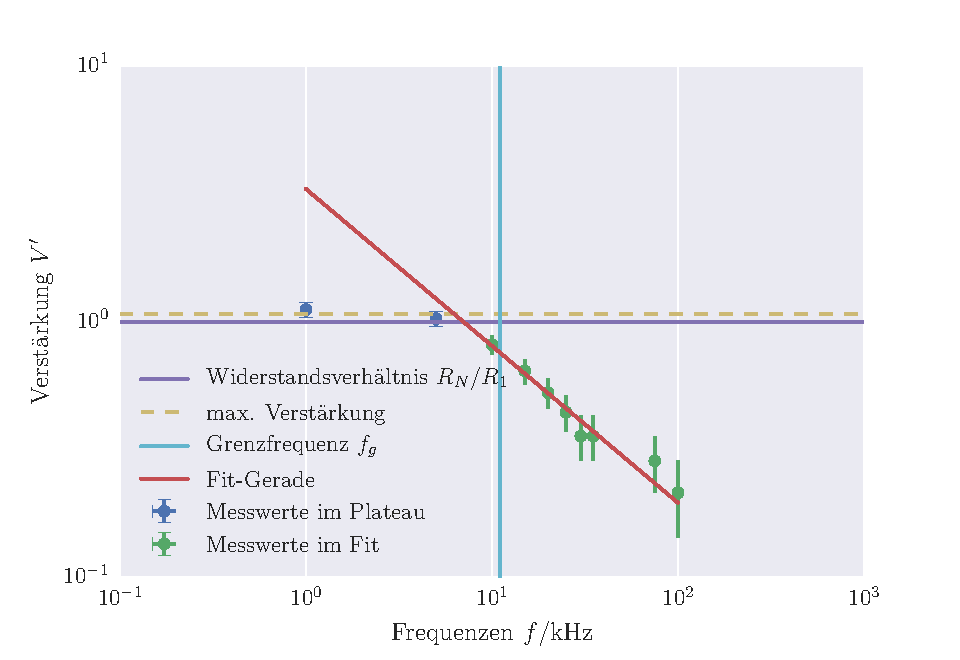
\includegraphics[scale=1]{../Grafiken/Gegengekoppelter_Verstaerker_1.pdf}
\caption{\label{fig:gegengekoppelter_verstaerker_1}}
\end{figure}
\FloatBarrier

\begin{table}[!h]
	\centering
	\begin{tabular}{ccc}
		\toprule
		Frequenz & Ausgangsspannung & Ausgangsspannung\\
		$f$/\si{\hertz} & $U_{A,\mathrm{int}}$/\si{\milli\volt} & $U_{A,\mathrm{diff}}$/\si{\milli\volt}\\
\midrule
		\num{100(1)} & \num{670(10)} & \num{140(10)}\\
		\num{200(2)} & \num{350(10)} & \num{240(10)}\\
		\num{300(3)} & \num{250(10)} & \num{350(10)}\\
		\num{400(4)} & \num{180(10)} & \num{450(10)}\\
		\num{500(5)} & \num{160(10)} & \num{550(10)}\\
		\num{600(6)} & \num{140(10)} & \num{640(10)}\\
		\num{700(7)} & \num{120(10)} & \num{740(10)}\\
		\num{800(8)} & \num{100(10)} & \num{840(10)}\\
		\num{900(9)} & \num{90(10)} & \num{920(10)}\\
		\num{1000(10)} & \num{80(10)} & \num{1040(10)}\\
		\bottomrule
	\end{tabular}
	\caption{ Messwerte der Frequenz der Eingangsspannung und der Ausgangsspannung für die Schaltungen eines Umkehrintegrators und -differentiators. \label{tab:integrator_differentiator}}
\end{table}

\FloatBarrier
\begin{figure}[!h]
\centering
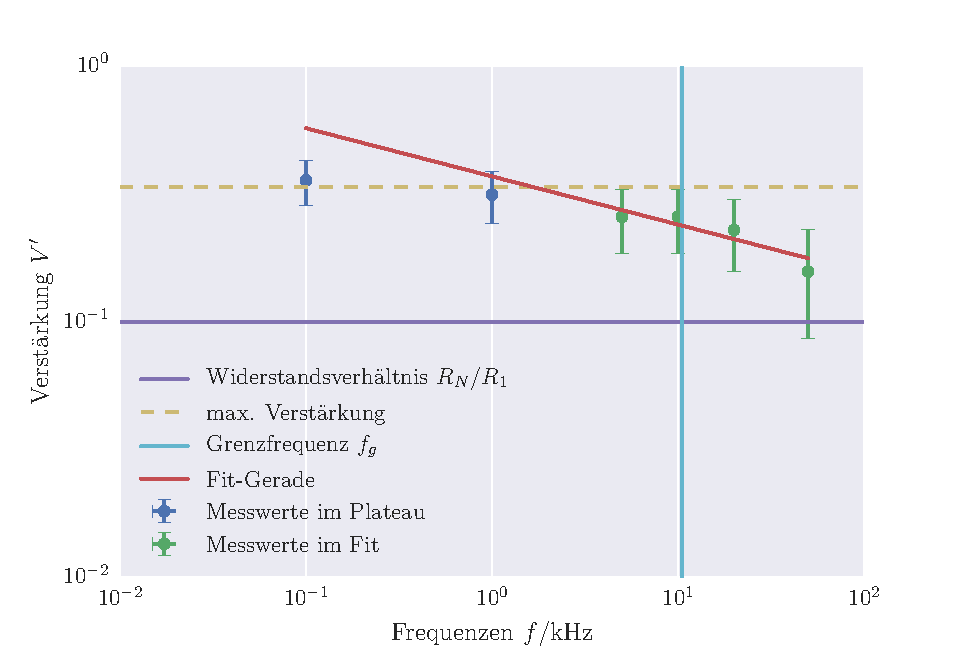
\includegraphics[scale=1]{../Grafiken/Gegengekoppelter_Verstaerker_2.pdf}
\caption{\label{fig:gegengekoppelter_verstaerker_2}}
\end{figure}
\FloatBarrier

\begin{table}[!h]
	\centering
	\begin{tabular}{ccc}
		\toprule
		Frequenz & Ausgangsspannung & Verstärkung\\
		$f$/\si{\kilo\hertz} & $U_{\mathrm{A}}$/\si{\milli\volt} & $V$\\
\midrule
		\num{0.0100(1)} & \num{37(5)} & \num{0.53(7)}\\
		\num{0.100(1)} & \num{35(5)} & \num{0.50(7)}\\
		\num{1.00(1)} & \num{38(5)} & \num{0.54(7)}\\
		\num{10.0(1)} & \num{32(5)} & \num{0.46(7)}\\
		\num{20.0(2)} & \num{30(5)} & \num{0.43(7)}\\
		\num{30.0(3)} & \num{25(5)} & \num{0.36(7)}\\
		\num{40.0(4)} & \num{19(5)} & \num{0.27(7)}\\
		\num{50.0(5)} & \num{19(5)} & \num{0.27(7)}\\
		\num{100(1)} & \num{16(5)} & \num{0.23(7)}\\
		\bottomrule
	\end{tabular}
	\caption{Messwerte der Frequenz und der Ausgangsspannung der dritten Schaltung eines gegengekoppelten Verstärkers.
            Zusätzlich ist die Verstärkung dieser Schaltung angegeben. \label{tab:gegengekoppelter_verstaerker_3}}
\end{table}

\FloatBarrier
\begin{figure}[!h]
\centering
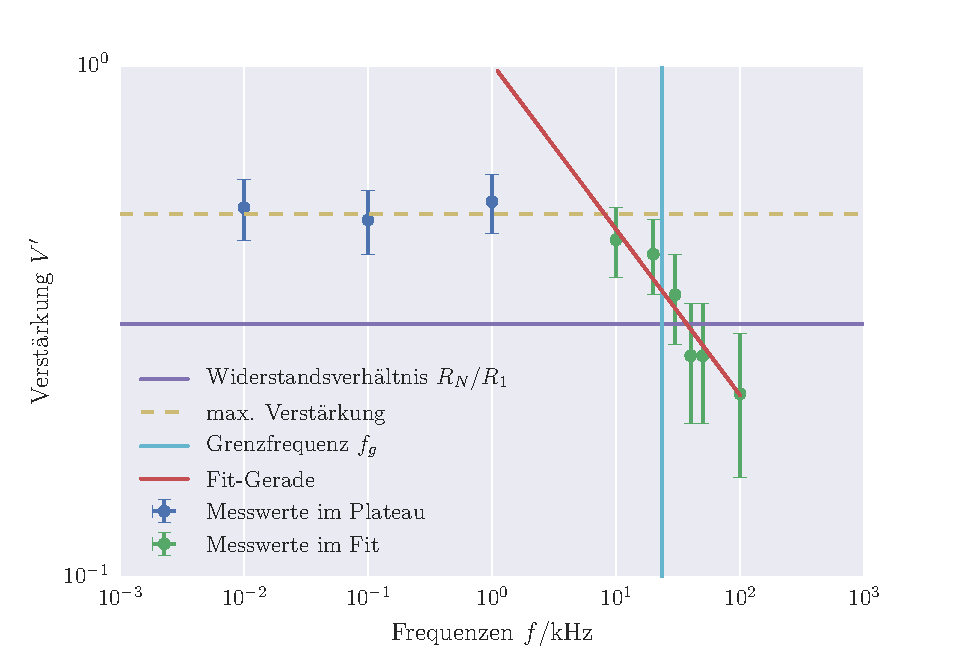
\includegraphics[scale=1]{../Grafiken/Gegengekoppelter_Verstaerker_3.pdf}
\caption{Doppellogarithmische Darstellung der Verstärkung der dritten gegengekoppelten Verstärkerschaltung in Abhängigkeit der Frequenz der Eingangsspannug. Zusätzlich wurden die Ausgleichsgerade
	durch die abfallenden Messwerte und eine senkrechte Gerade bei der Grenzfrequenz eingezeichnet. Ferner sind noch  zwei waagerechte Geraden dargestellt. Die eine markiert den Mittelwert der Messwerte im Plateau und die  andere
	den theoretischen Wert dieser Größe.\label{fig:gegengekoppelter_verstaerker_3}}
\end{figure}
\FloatBarrier

\begin{table}[!h]
	\centering
	\begin{tabular}{ccc}
		\toprule
		Frequenz & Ausgangsspannung & Verstärkung\\
		$f$/\si{\kilo\hertz} & $U_A$/\si{\milli\volt} & $V$\\
\midrule
		\num{0.100(1)} & \num{220(5)} & \num{3.14(8)}\\
		\num{1.00(1)} & \num{230(5)} & \num{3.29(9)}\\
		\num{5.00(5)} & \num{160(5)} & \num{2.29(8)}\\
		\num{10.0(1)} & \num{100(5)} & \num{1.43(7)}\\
		\num{20.0(2)} & \num{60(5)} & \num{0.86(7)}\\
		\num{30.0(3)} & \num{45(5)} & \num{0.64(7)}\\
		\num{50.0(5)} & \num{35(5)} & \num{0.50(7)}\\
		\num{100(1)} & \num{25(5)} & \num{0.36(7)}\\
		\bottomrule
	\end{tabular}
	\caption{Messwerte der Frequenz und der Ausgangsspannung der vierten Schaltung eines gegengekoppelten Verstärkers.
            Zusätzlich ist die Verstärkung dieser Schaltung angegeben. \label{tab:gegengekoppelter_verstaerker_4}}
\end{table}

\FloatBarrier
\begin{figure}[!h]
\centering
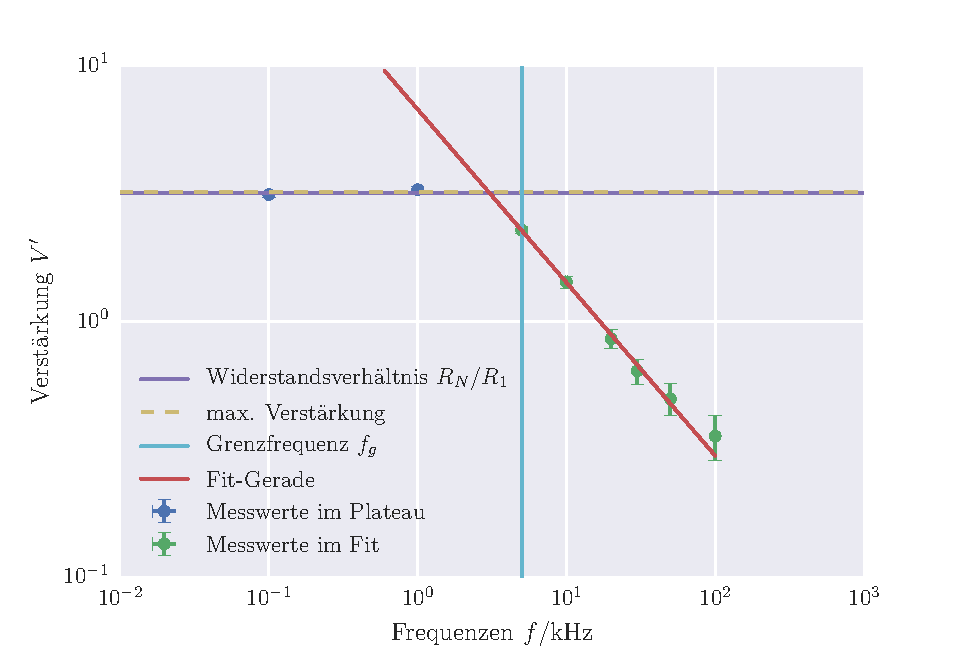
\includegraphics[scale=1]{../Grafiken/Gegengekoppelter_Verstaerker_4.pdf}
\caption{\label{fig:gegengekoppelter_verstaerker_4}}
\end{figure}
\FloatBarrier


\begin{table}[!h]
	\centering
	\begin{tabular}{cc}
		\toprule
		Frequenz & Phase\\
		$f$/\si{\kilo\hertz} & $\Delta \phi$/\si{\degree}\\
\midrule
		\num{0.100(1)} & \num{175(5)}\\
		\num{0.200(2)} & \num{170(5)}\\
		\num{0.300(3)} & \num{168(5)}\\
		\num{0.400(4)} & \num{168(5)}\\
		\num{0.500(5)} & \num{165(5)}\\
		\num{1.00(1)} & \num{162(5)}\\
		\num{2.00(2)} & \num{150(5)}\\
		\num{3.00(3)} & \num{140(5)}\\
		\num{4.00(4)} & \num{130(5)}\\
		\num{5.00(5)} & \num{125(5)}\\
		\num{10.0(1)} & \num{110(5)}\\
		\num{20.0(2)} & \num{90(5)}\\
		\bottomrule
	\end{tabular}
	\caption{Messwerte der Frequenz und der Phase zwischen Eingangs- und Ausgangsspannung der vierten Schaltung 
eines gegengekoppelten Verstärkers. \label{tab:gegengekoppelter_verstaerker_phase}}
\end{table}

\FloatBarrier
\begin{figure}[!h]
\centering
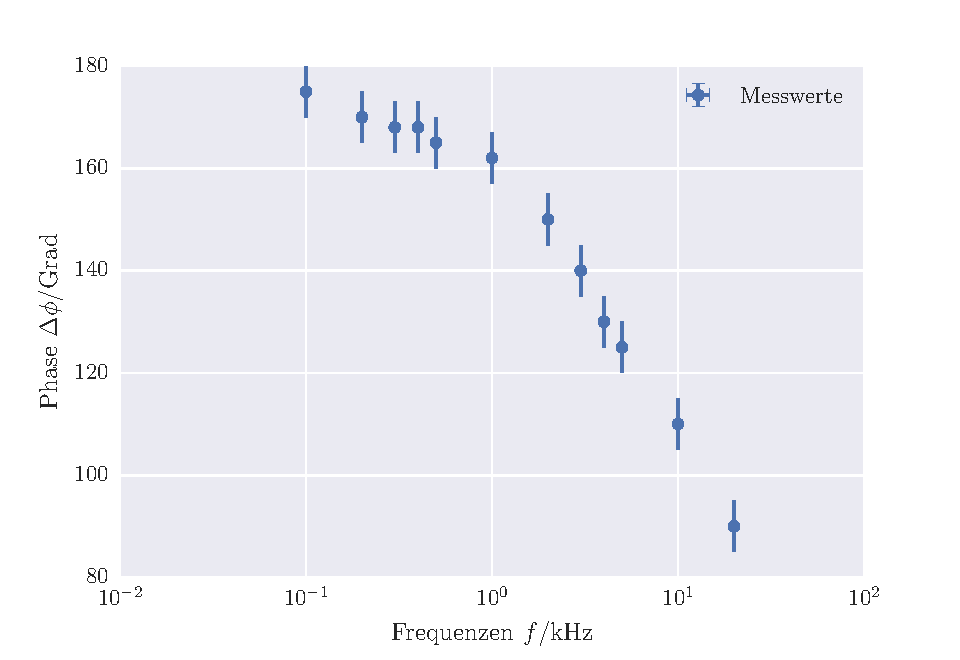
\includegraphics[scale=1]{../Grafiken/Gegengekoppelter_Verstaerker_Phase.pdf}
\caption{\label{fig:gegengekoppelter_verstaerker_phase}}
\end{figure}
\FloatBarrier



\subsection{Amperemeter mit geringem Eingangswiderstand}
\begin{table}[!h]
	\centering
	\begin{adjustbox}{width=1\textwidth}
	\begin{tabular}{cccccc}
		\toprule
		Frequenz & Generatorspannung & Eingangsspannung & Ausgangsspannung & Ausgangsspannung & Ausgangsspannung\\
		$f$/\si{\kilo\hertz} & $U_{\mathrm{g}}$/\si{\milli\volt} & $U_{\mathrm{E}}$/\si{\milli\volt} & $U_{\mathrm{A}}$/\si{\volt} & $U_{\mathrm{A},\mathrm{theo}}$/\si{\volt} & $\Delta_{\mathrm{rel}}U_{\mathrm{A}}$/\si{\percent}\\
\midrule
		\num{100(1)} & \num{0.209(1)} & \num{0.023(2)} & \num{20.0(1)} & \num{20.9(3)} & \num{4(2)}\\
		\num{200(2)} & \num{0.207(1)} & \num{0.023(2)} & \num{20.0(1)} & \num{20.7(3)} & \num{3(2)}\\
		\num{500(5)} & \num{0.207(1)} & \num{0.030(2)} & \num{20.0(1)} & \num{20.7(3)} & \num{3(2)}\\
		\num{750(8)} & \num{0.207(1)} & \num{0.035(2)} & \num{20.0(1)} & \num{20.7(3)} & \num{3(2)}\\
		\num{1000(10)} & \num{0.207(1)} & \num{0.040(2)} & \num{20.0(1)} & \num{20.7(3)} & \num{3(2)}\\
		\num{1500(15)} & \num{0.207(1)} & \num{0.050(2)} & \num{19.0(1)} & \num{20.7(3)} & \num{8(2)}\\
		\num{2000(20)} & \num{0.207(1)} & \num{0.060(2)} & \num{19.0(1)} & \num{20.7(3)} & \num{8(2)}\\
		\num{2500(25)} & \num{0.207(1)} & \num{0.075(2)} & \num{19.5(1)} & \num{20.7(3)} & \num{6(2)}\\
		\num{3000(30)} & \num{0.207(1)} & \num{0.085(2)} & \num{19.5(1)} & \num{20.7(3)} & \num{6(2)}\\
		\num{3500(35)} & \num{0.207(1)} & \num{0.095(2)} & \num{19.5(1)} & \num{20.7(3)} & \num{6(2)}\\
		\num{4000(40)} & \num{0.207(1)} & \num{0.105(2)} & \num{18.0(1)} & \num{20.7(3)} & \num{14(2)}\\
		\num{4500(45)} & \num{0.207(1)} & \num{0.110(2)} & \num{18.7(1)} & \num{20.7(3)} & \num{10(2)}\\
		\num{5000(50)} & \num{0.207(1)} & \num{0.125(2)} & \num{18.3(1)} & \num{20.7(3)} & \num{13(2)}\\
		\num{5500(55)} & \num{0.207(1)} & \num{0.140(2)} & \num{18.0(1)} & \num{20.7(3)} & \num{14(2)}\\
		\num{6000(60)} & \num{0.207(1)} & \num{0.150(2)} & \num{17.5(1)} & \num{20.7(3)} & \num{18(2)}\\
		\num{6500(65)} & \num{0.207(1)} & \num{0.160(2)} & \num{17.3(1)} & \num{20.7(3)} & \num{19(2)}\\
		\num{7000(70)} & \num{0.207(1)} & \num{0.170(2)} & \num{16.9(1)} & \num{20.7(3)} & \num{22(2)}\\
		\num{7500(75)} & \num{0.207(1)} & \num{0.185(2)} & \num{16.5(1)} & \num{20.7(3)} & \num{25(2)}\\
		\num{8500(85)} & \num{0.207(1)} & \num{0.195(2)} & \num{16.3(1)} & \num{20.7(3)} & \num{26(2)}\\
		\num{9000(90)} & \num{0.207(1)} & \num{0.200(2)} & \num{15.7(1)} & \num{20.7(3)} & \num{31(2)}\\
		\num{10000(100)} & \num{0.207(1)} & \num{0.215(2)} & \num{14.7(1)} & \num{20.7(3)} & \num{40(2)}\\
		\bottomrule
	\end{tabular}
\end{adjustbox}
	\caption{ Messwerte der Frequenz der Eingangsspannung, der Generator-, der Eingangs- und Ausgangsspannung
der Ampermeterschaltung. Zusätzlich ist die theoretische Ausgangsspannung und der realtive Unterschied zwischen dieser
und der gemessenen angegeben. \label{tab:amperemeter_1}}
	
\end{table}


\begin{table}[!h]
	\centering
	\begin{tabular}{cccc}
		\toprule
		Frequenz & Strom & Eingangswiderstad & Leerlaufverstärkung\\
		$f$/\si{\kilo\hertz} & $I$/\si{\ampere} & $r_{\mathrm{e}}$/\si{\ohm} & $V$\\
\midrule
		\num{100(1)} & \num{0.00209(2)} & \num{11(1)} & \num{908(80)}\\
		\num{200(2)} & \num{0.00207(2)} & \num{11(1)} & \num{899(79)}\\
		\num{500(5)} & \num{0.00207(2)} & \num{14(1)} & \num{690(47)}\\
		\num{750(8)} & \num{0.00207(2)} & \num{16(1)} & \num{591(35)}\\
		\num{1000(10)} & \num{0.00207(2)} & \num{19(1)} & \num{517(27)}\\
		\num{1500(15)} & \num{0.00207(2)} & \num{24(1)} & \num{413(18)}\\
		\num{2000(20)} & \num{0.00207(2)} & \num{28(1)} & \num{345(13)}\\
		\num{2500(25)} & \num{0.00207(2)} & \num{36(1)} & \num{276(8)}\\
		\num{3000(30)} & \num{0.00207(2)} & \num{41(1)} & \num{243(7)}\\
		\num{3500(35)} & \num{0.00207(2)} & \num{45(1)} & \num{217(6)}\\
		\num{4000(40)} & \num{0.00207(2)} & \num{50(1)} & \num{197(5)}\\
		\num{4500(45)} & \num{0.00207(2)} & \num{53(1)} & \num{188(4)}\\
		\num{5000(50)} & \num{0.00207(2)} & \num{60(1)} & \num{165(4)}\\
		\num{5500(55)} & \num{0.00207(2)} & \num{67(1)} & \num{147(3)}\\
		\num{6000(60)} & \num{0.00207(2)} & \num{72(1)} & \num{138(3)}\\
		\num{6500(65)} & \num{0.00207(2)} & \num{77(1)} & \num{129(2)}\\
		\num{7000(70)} & \num{0.00207(2)} & \num{82(1)} & \num{121(2)}\\
		\num{7500(75)} & \num{0.00207(2)} & \num{89(1)} & \num{111(2)}\\
		\num{8500(85)} & \num{0.00207(2)} & \num{94(1)} & \num{106(2)}\\
		\num{9000(90)} & \num{0.00207(2)} & \num{96(1)} & \num{103(2)}\\
		\num{10000(100)} & \num{0.00207(2)} & \num{103(1)} & \num{96(2)}\\
		\bottomrule
	\end{tabular}
	\caption{ Aus den gemessenen Spannungen der Amperemeterschaltung berechnete Werte des Stroms und des Eingangswiderstands
sowie die aus letzterem berechneten Werte der Leerlaufverstärkung. \label{tab:amperemeter_2}}
\end{table}


\FloatBarrier
\begin{figure}[!h]
\centering
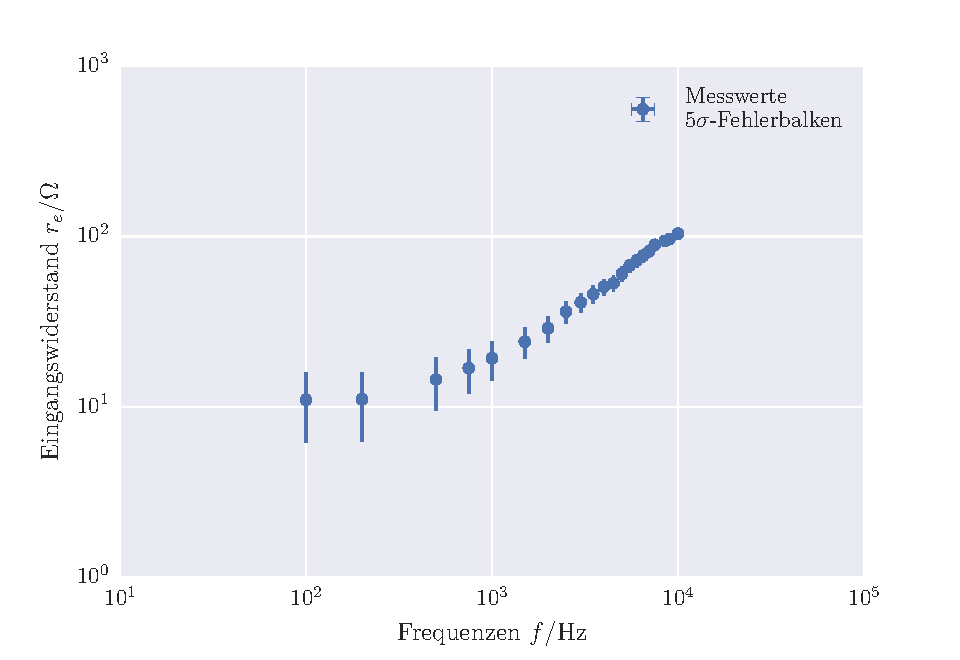
\includegraphics[scale=1]{../Grafiken/Amperemeter_Eingangswiderstand.pdf}
\caption{Doppellogarithmische Darstellung des Eingangswiderstands der Amperemeterschaltung
	in Abhängigkeit der Frequenz. \label{fig:amperemeter_eingangswiderstand}}
\end{figure}
\FloatBarrier
\FloatBarrier
\begin{figure}[!h]
\centering
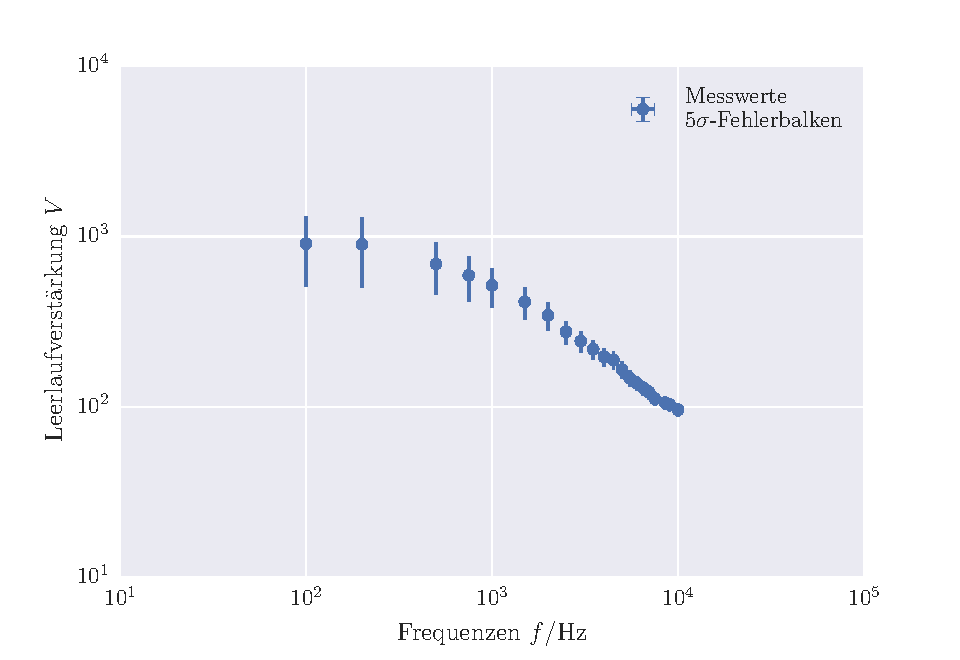
\includegraphics[scale=1]{../Grafiken/Amperemeter_Leerlaufverstaerkung.pdf}
\caption{Doppellogarithmische Darstellung des Leerlaufverstärkung der Amperemeterschaltung
	in Abhängigkeit der Frequenz.  \label{fig:amperemeter_leerlaufverstaerkung}}
\end{figure}
\FloatBarrier

\subsection{Integrator- und Differentiatorschaltung}
\begin{table}[!h]
	\centering
	\begin{tabular}{ccc}
		\toprule
		Frequenz & Ausgangsspannung & Ausgangsspannung\\
		$f$/\si{\hertz} & $U_{A,\mathrm{int}}$/\si{\milli\volt} & $U_{A,\mathrm{diff}}$/\si{\milli\volt}\\
\midrule
		\num{100(1)} & \num{670(10)} & \num{140(10)}\\
		\num{200(2)} & \num{350(10)} & \num{240(10)}\\
		\num{300(3)} & \num{250(10)} & \num{350(10)}\\
		\num{400(4)} & \num{180(10)} & \num{450(10)}\\
		\num{500(5)} & \num{160(10)} & \num{550(10)}\\
		\num{600(6)} & \num{140(10)} & \num{640(10)}\\
		\num{700(7)} & \num{120(10)} & \num{740(10)}\\
		\num{800(8)} & \num{100(10)} & \num{840(10)}\\
		\num{900(9)} & \num{90(10)} & \num{920(10)}\\
		\num{1000(10)} & \num{80(10)} & \num{1040(10)}\\
		\bottomrule
	\end{tabular}
	\caption{ Messwerte der Frequenz der Eingangsspannung und der Ausgangsspannung für die Schaltungen eines Umkehrintegrators und -differentiators. \label{tab:integrator_differentiator}}
\end{table}


\FloatBarrier
\begin{figure}[!h]
\centering
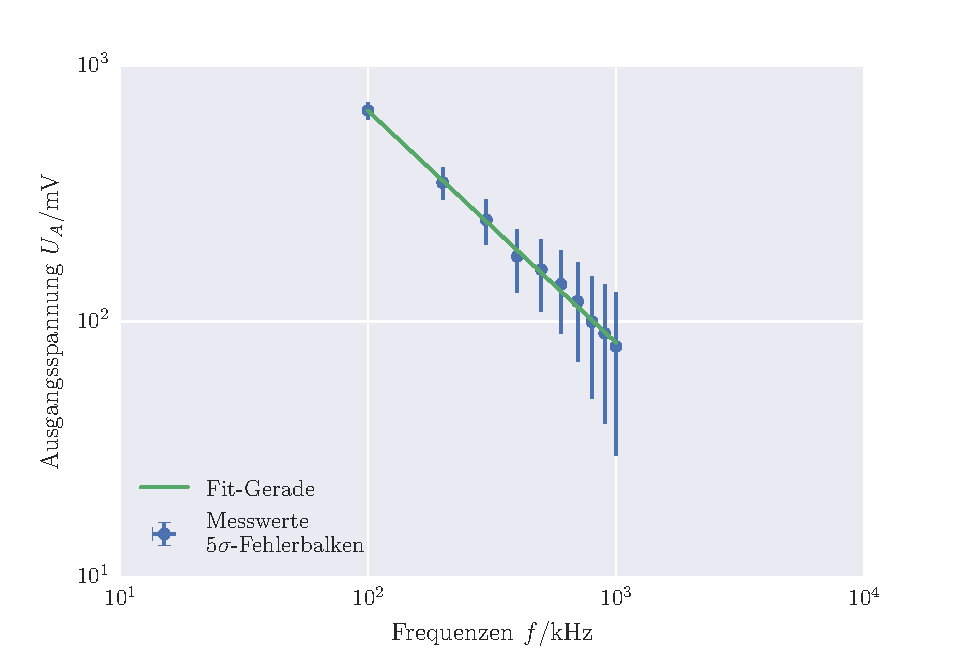
\includegraphics[scale=1]{../Grafiken/Integrator_Frequenz.pdf}
\caption{\label{fig:integrator_frequenz}}
\end{figure}
\FloatBarrier
\FloatBarrier
\begin{figure}[!h]
\centering
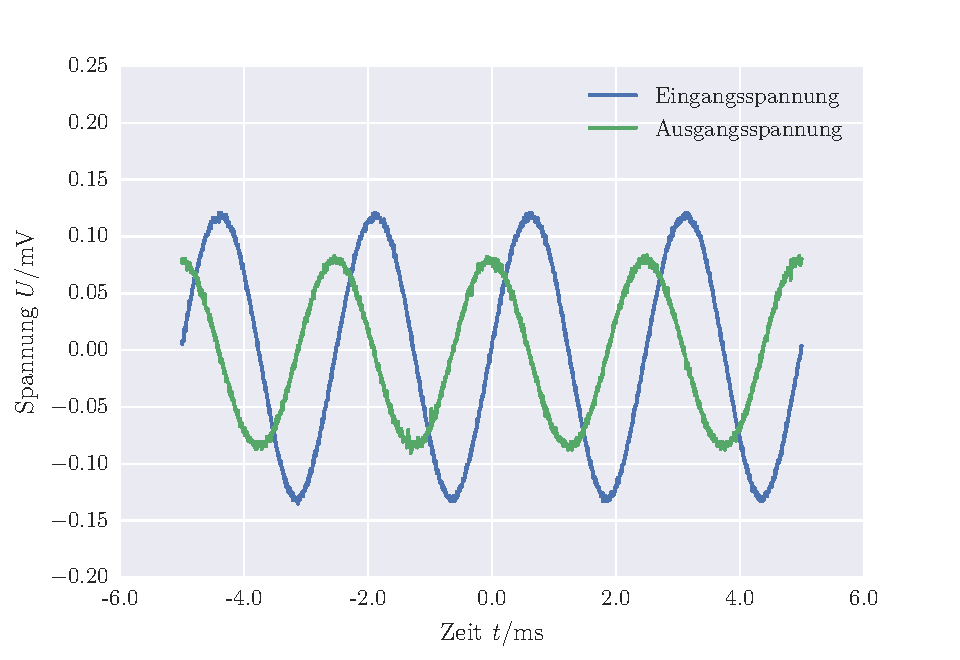
\includegraphics[scale=1]{../Grafiken/Integrator_Oszilloskop_Sinus.pdf}
\caption{Vom Oszilloskop aufgenommene Ein- und Ausgangsspannungen der Integratorschaltung. Auf dem Eingang
	liegt hier eine Sinusspannung. \label{fig:integrator_oszilloskop_sinus}}
\end{figure}
\FloatBarrier
\FloatBarrier
\begin{figure}[!h]
\centering
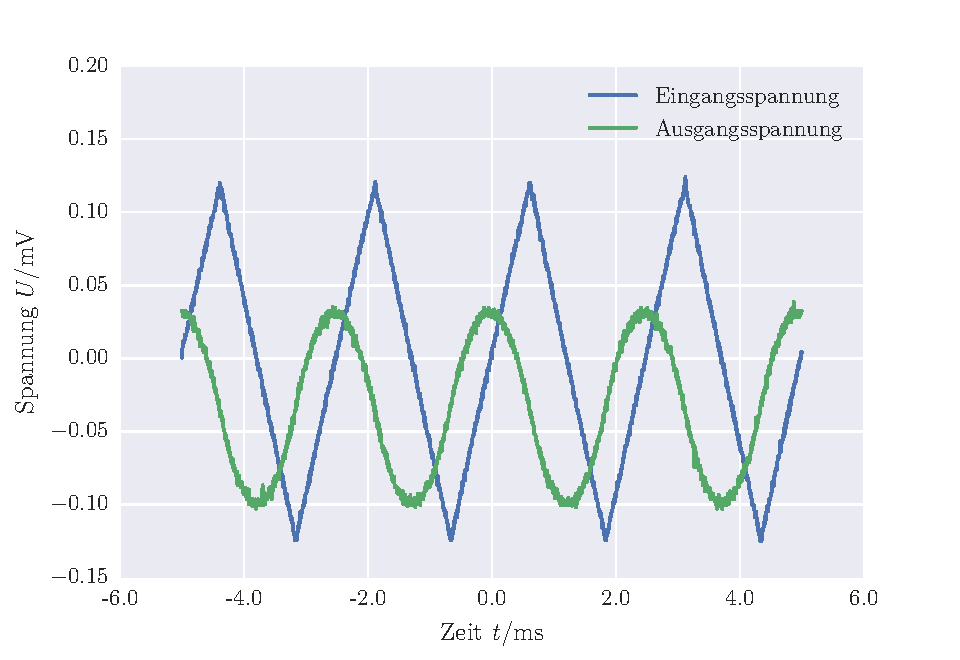
\includegraphics[scale=0.75]{../Grafiken/Integrator_Oszilloskop_Dreieck.pdf}
\caption{Vom Oszilloskop aufgenommene Ein- und Ausgangsspannungen der Integratorschaltung. Auf dem Eingang
	liegt hier eine Dreicksspannung. Die Ausgangsspannung in Parabelform entspricht dem theoretisch
	zu erwartendem Verlauf (periodische Abfolge nach oben respektive nach unten geöffneter 
	Parabeln).\label{fig:integrator_oszilloskop_dreieck}}
\end{figure}
\FloatBarrier
\FloatBarrier
\begin{figure}[!h]
\centering
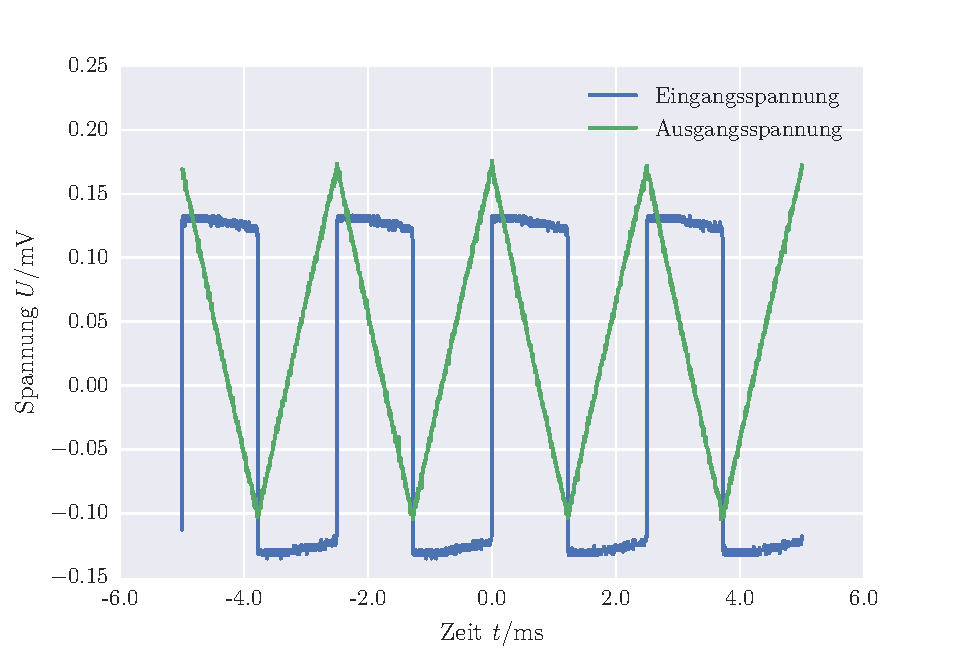
\includegraphics[scale=0.75]{../Grafiken/Integrator_Oszilloskop_Rechteck.pdf}
\caption{Vom Oszilloskop aufgenommene Ein- und Ausgangsspannungen der Integratorschaltung. Auf dem Eingang
	liegt hier eine Rechteckspannung.  Die Ausgangsspannung in Form einer Dreieckspannung entspricht dem theoretisch
	zu erwartendem Verlauf.\label{fig:integrator_oszilloskop_rechteck}}
\end{figure}
\FloatBarrier
\FloatBarrier
\begin{figure}[!h]
\centering
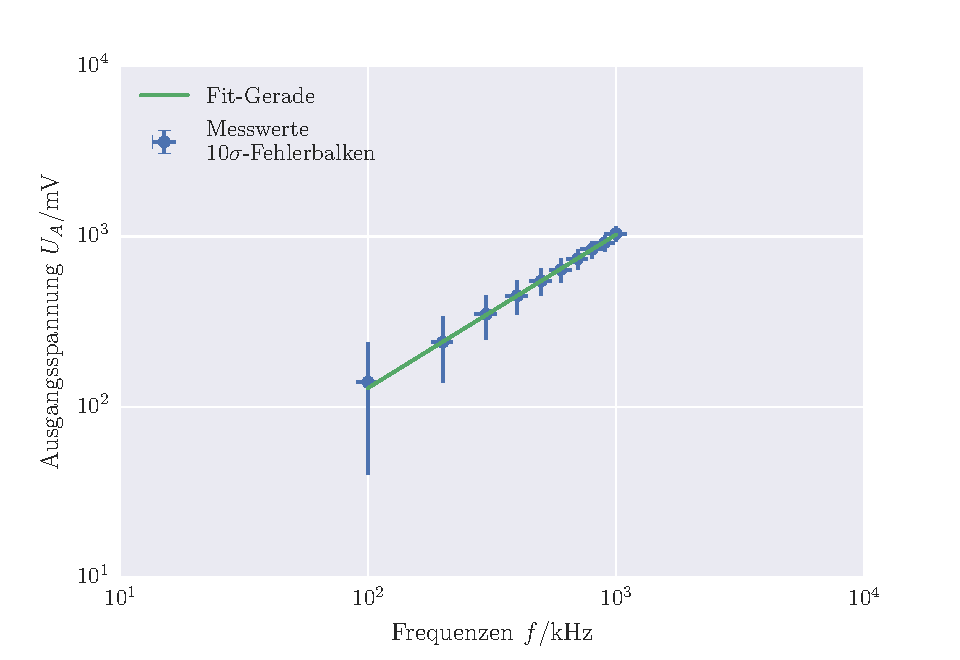
\includegraphics[scale=1]{../Grafiken/Differentiator_Frequenz.pdf}
\caption{\label{fig:differentiator_frequenz}}
\end{figure}
\FloatBarrier
\FloatBarrier
\begin{figure}[!h]
\centering
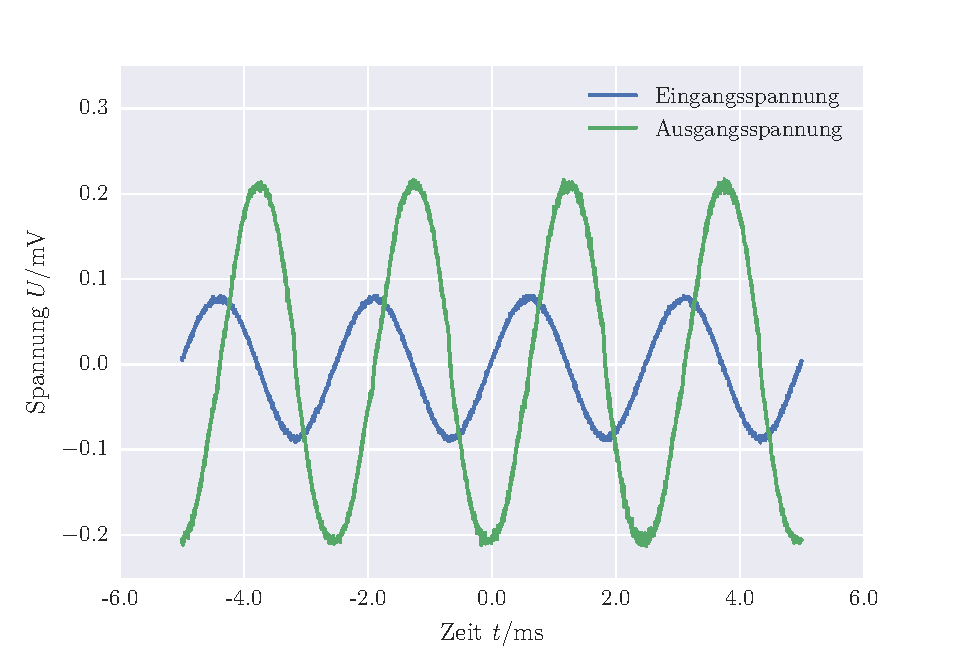
\includegraphics[scale=0.75]{../Grafiken/Differentiator_Oszilloskop_Sinus.pdf}
\caption{Vom Oszilloskop aufgenommene Ein- und Ausgangsspannungen der Differentiatorschaltung. Auf dem Eingang
	liegt hier eine Sinusspannung.\label{fig:differentiator_oszilloskop_sinus}}
\end{figure}
\FloatBarrier
\FloatBarrier
\begin{figure}[!h]
\centering
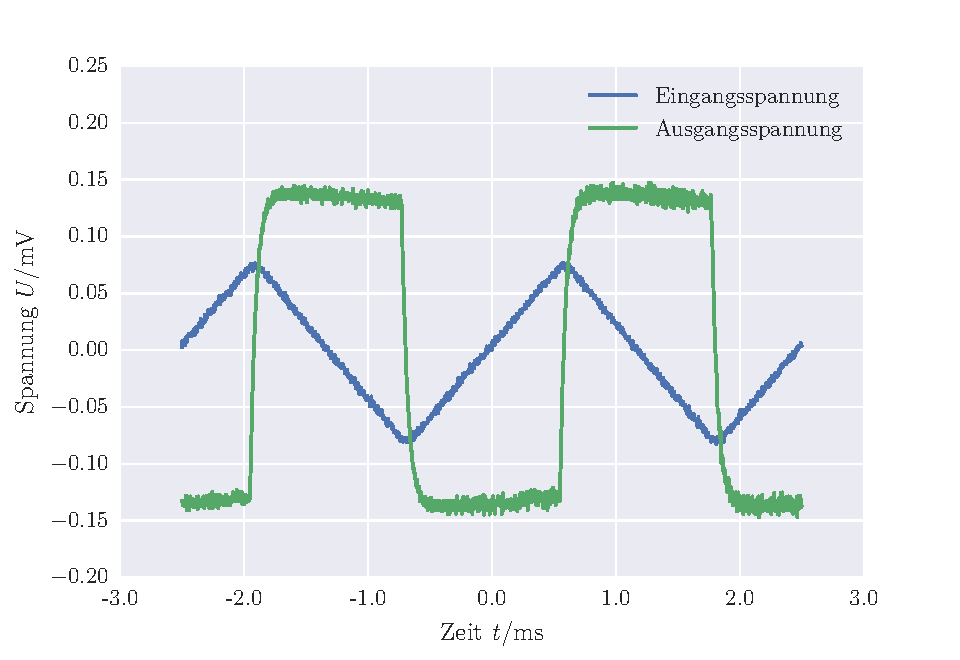
\includegraphics[scale=1]{../Grafiken/Differentiator_Oszilloskop_Dreieck.pdf}
\caption{\label{fig:differentiator_oszilloskop_dreieck}}
\end{figure}
\FloatBarrier
\FloatBarrier
\begin{figure}[!h]
\centering
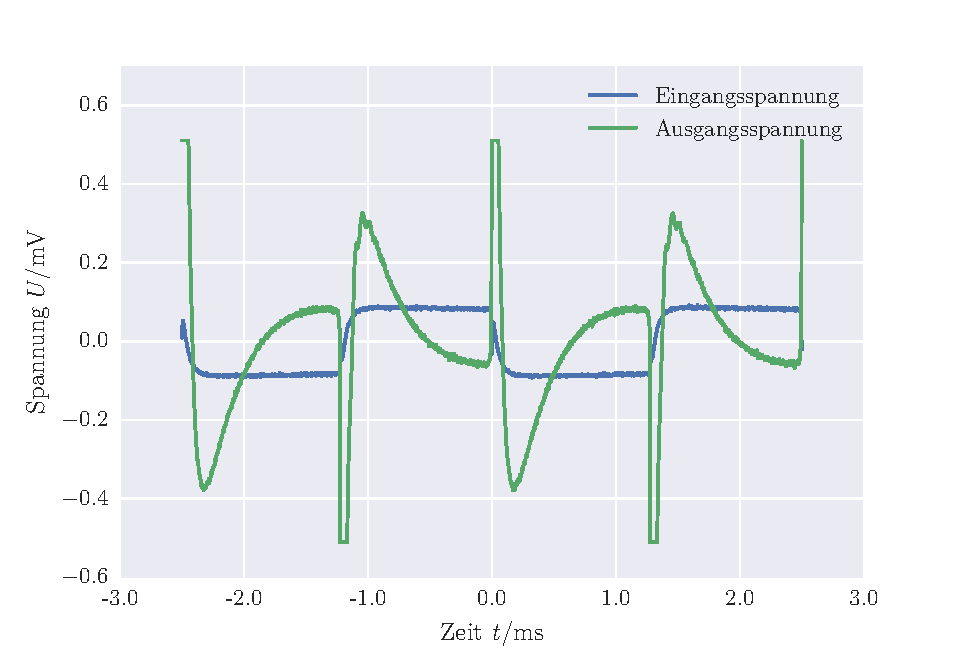
\includegraphics[scale=0.75]{../Grafiken/Differentiator_Oszilloskop_Rechteck.pdf}
\caption{Vom Oszilloskop aufgenommene Ein- und Ausgangsspannungen der Differentiatorschaltung. Auf dem Eingang
	liegt hier eine Rechteckspannung. Die Ausgangsspannung in Form schmalen hohen Peaks entspricht in etwa dem 
	theoretisch zu erwartendem Verlauf eines Delta-Kamms.\label{fig:differentiator_oszilloskop_rechteck}}
\end{figure}
\FloatBarrier

\subsection{Schmitt-Trigger}

\subsection{Funktionsgenerator}

\FloatBarrier
\begin{figure}[!h]
\centering
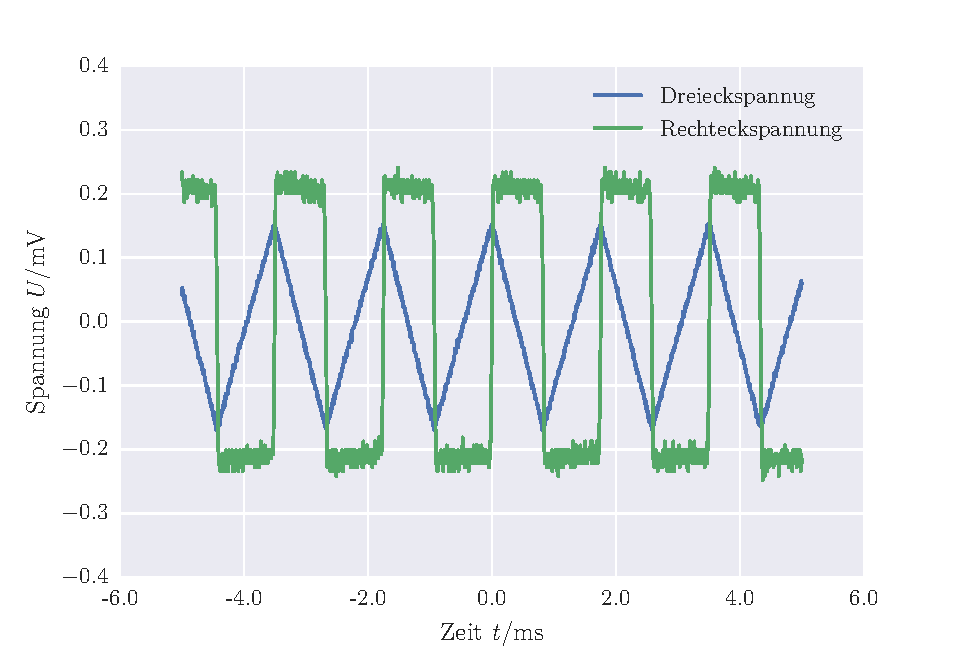
\includegraphics[scale=1]{../Grafiken/Funktionsgenerator.pdf}
\caption{Vom Oszilloskop aufgenommene Rechteck- und Dreiecksspannung der Funktionsgeneratorschaltung.\label{fig:funktionsgenerator}}
\end{figure}
\FloatBarrier



